\documentclass{report}
\usepackage[utf8]{inputenc}
\usepackage[T1]{fontenc}
\usepackage{amsmath}
\usepackage{amssymb,amsfonts,textcomp}
\usepackage{array}
\usepackage{hhline}
\usepackage{hyperref}
\hypersetup{colorlinks=true, linkcolor=blue, citecolor=blue, filecolor=blue, urlcolor=blue, pdftitle=, pdfauthor=Gilles Vuidel, pdfsubject=, pdfkeywords=}
\usepackage{graphicx}
\usepackage[top=2.501cm,bottom=2.501cm,left=2.501cm,right=2.501cm,nohead]{geometry}
\usepackage{float}
\usepackage{parskip}
\usepackage{multirow}
\usepackage{caption}
\usepackage{fancyvrb}
\makeatletter
\newcommand\arraybslash{\let\\\@arraycr}
\makeatother
% centering figures
\makeatletter
\g@addto@macro\@floatboxreset\centering
\makeatother
\setlength\tabcolsep{1mm}
\renewcommand\arraystretch{1.3}

% saut de page après une section
%\let\oldsection\section
%\renewcommand\section{\clearpage\oldsection}

% saut après itemize
\let\EndItemize\enditemize
\def\enditemize{\EndItemize\medskip}

\begin{document}
 \begin{titlepage}
	
	\centering
	
\includegraphics[scale=0.5]{img/logo.png}\\
	
	\bigskip
	\bigskip
	\bigskip	
	{\Huge
		\bfseries
		PixScape 1.0\\
		\bigskip
		User manual\\
	}
	\bigskip
	\bigskip
	\bigskip
	\bigskip
	\bigskip
	
	{\Large		
		Gilles Vuidel, Yohan Sahraoui et Jean-Christophe Foltête\\
		\bigskip
		2017-03-21\\
	}
	
\end{titlepage}

\setcounter{tocdepth}{2}
%\renewcommand\contentsname{}
\tableofcontents

\pagebreak

\chapter{Introduction}

\section{About PixScape}

PixScape software is dedicated to the analysis of the landscape visibility from raster data.
This software integrates the main functionalities available in standard GIS  in this domain and offers other original features such as tangential view and multi-resolution analysis.


\subsection{Authors}
PixScape has been developed at \href{http://thema.univ-fcomte.fr}{ThéMA} laboratory (\href{http://www.univ-fcomte.fr}{Université de Franche-Comté} – \href{http://www.cnrs.fr}{CNRS}) by Gilles Vuidel in collaboration with Jean-Christophe Foltête, Daniel Joly, Yohan Sahraoui et Samy Youssoufi. The PixScape logo has been designed by Xavier Girardet.

\subsection{Terms of use}
Graphab is distributed in open source, under the \href{https://www.gnu.org/licenses/gpl-3.0.html}{GPL} license.\\
Source code can be downloaded from the sourcesup git repository : \url{git://git.renater.fr/pixscape.git}.\\
Users must cite the following reference in their publications :\\
??


\section{System requirements}

PixScape runs on any computer supporting Java 7 or later (PC under Linux, Windows, Mac, ...). 
However, when dealing with large datasets, the amount of memory (RAM) will limit the maximum area that can be processed. In addition, processing power (CPU) will determine the speed of computing. For details, see section \nameref{perf}.

For GPU computing, PixScape supports only Nvidia graphics card with CUDA. By default, PixScape is compiled with CUDA 6.5. If you cannot install CUDA 6.5, you will need to install the JCuda library corresponding to your CUDA version and launch PixScape in command line (see \nameref{cuda}). JCuda binaries are available here: \href{http://www.jcuda.org/downloads/downloads.html}{www.jcuda.org/downloads/downloads.html}

\section{Installation and launching PixScape}

PixScape is available for downloading at : \url{http://sourcesup.renater.fr/pixscape}.

\begin{itemize}
	\item Download and install Java 7 or later (\href{http://www.java.com}{java.com}). It is best to install 64 bits version of Java.
	\item Download pixscape-1.0.jar
	\item Launch pixscape-1.0.jar
\end{itemize}

PixScape can be used through 2 user interface : the graphical user interface (GUI) and the command line interface (CLI).

The graphical user interface allows to create project, visualize the data, calculate interactively viewsheds and visibility metrics, and perform exhaustive visibility metric calculation on local computer. The command line interface allows to run the same calculations on remote computers as well as on computer clusters.

The following chapter (\ref{gui}) describes all of the software features available from the GUI. Chapter \ref{cli} details how to use PixScape on the command line. Chapter \ref{principles} explains how visibility calculations are implemented in PixScape. The set of available metrics is detailed in Chapter \ref{metrics}. And Chapter \ref{perf} reviews the parallelization modes, performance and memory management.


\chapter{Graphical user interface (GUI)}
\label{gui}

Once PixScape is launched, the first step is to create a project based on a DTM (Digital Terrain Model) covering the studied area.

\section{Project creation}

To create a new project, use the menu File / New project. User must 
La mise en place d’un nouveau projet PixScape s’effectue à partir du menu : File / New project. User must enter a name and a path for the project as well as a DTM in Tiff or AsciiGrid format. \textbf{The coordinate system of the DTM must be projected and in meter unit. If this is not the case, the visibility calculations will be erroneous.} The resolution of the altitudes (Z) can be specified if it is not in meter. For example, if the altitudes are given in centimeter, enter 0.01 in "Z resolution".

\begin{figure}[H]
	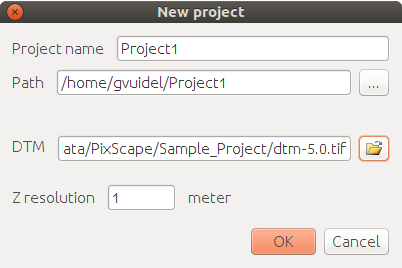
\includegraphics[scale=0.5]{img/new_project-en.png} 
	\caption{Creating a project}
\end{figure}

The created project stores in its folder, the DTM converted in Tiff format with altitudes in meter, and the XML file containing the project settings.
For opening a project, simply select the corresponding XML file from the File / Load Project menu.

The DTM is sufficient to perform visibility calculations, but it can be more interesting to add additional information to perform more accurate analyses.

\section{Data management}

For importing raster data, PixScape supports 2 file formats : Tiff and AsciiGrid.
For Tiff format, the coordinate system can be given by 2 ways : directly in the Tiff file with the GeoTiff extension, or an additional text file with the same name and extension .tfw.


\subsection{Additional layers}
Two additional raster layers can be added to an existing project: the DSM (Digital Surface Model) and the land use.

\subsubsection{DSM}
In PixScape, the DSM corresponds to the height of the object (building, trees, ...) on the ground. The addition of the DTM and the DSM makes it possible to obtain the total elevation of the elements of the landscape. 
The unit of heights must be expressed in meters. To load a DSM, simply select a raster file in Tiff or Asciigrid format from the Data / Load DSM menu. After loading, the DSM is stored in the project directory

\subsubsection{Land use}
The land use layer is used by several landscape configuration metrics (S, IJI, CONTAG, etc.). The codes for land use categories must be between 0 and 255. To load a land use layer, simply select a raster file in Tiff or Asciigrid format from the Data / Load Land Use menu. After loading, the layer is stored in the project directory.

The colors associated with the land use categories are set randomly, but can be changed in the style of the layer. Color changes are automatically saved in the project's XML file to be kept from one opening to the next.

\textbf{These two layers must have exactly the same geometry as the DTM: the same spatial extent and the same resolution.} 

\subsection{Multiscale}
It is possible to add data at coarser resolutions to speed up visibility calculations. This data can be generated directly in PixScape from the Data / Multi scale / Generate menu or imported from the Data / Multi scale / Add scale menu.

\subsubsection{Generate multiscale data}
Generation of a multiscale database can be done directly in PixScape. User must give the required resolutions separated by commas. By default the software proposes 4 resolutions separated by a factor of 3. If the resolution of the initial data is 1 meters, the software will propose the resolutions 3m, 9m, 27m and 81m.

\begin{figure}[H]
	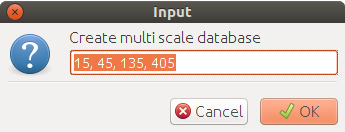
\includegraphics[scale=0.5]{img/gen_ms-en.png} 
	\caption{Multiscale database generation}
\end{figure}

It is recommended to use resolutions that follow a geometric sequence of a factor 2, 3 or 4.
PixScape will create a new DTM for each resolution, as well as the DSM and land use if these layers are present in the project.
For the DTM and the DSM the pixels are aggregated by the arithmetic mean, for the land use, the pixels are aggregated by the mode \ textit {ie.} the dominant land use category.
At the end of the processing, all the new layers are saved in Tiff format in the project directory and are added in the layer tree of the main window.


\subsubsection{Import data}
The multiscale database can be imported for each scale. At least DTM must be provided, and DSM plus landuse should be provided if these layers are already presents for the initial scale. As with the creation of the project, the resolution of the altitudes of the DTM can be indicated.

\begin{figure}[H]
	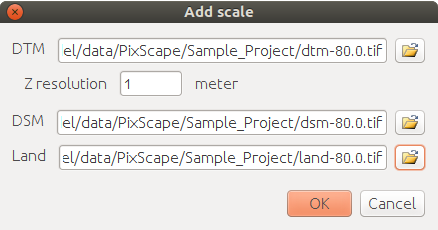
\includegraphics[scale=0.5]{img/add_scale-en.png} 
	\caption{Import layers for one scale}
\end{figure}

The resolution of the DSM heights must be in meters and the land use codes must be between 0 and 255. For land use, codes may vary from one scale to another to differentiate objects that do not have the same meaning according to the resolution, for example a tree and a forest, a building and a village.
The three layers must have exactly the same geometry: the same spatial extent and the same resolution.
Finally, the spatial extent must cover at least the spatial extent of the initial data.

When the project contains multiscale data, it can be used in visibility calculations by activating the multiscale setting in the Options window (see \nameref{options}).


\section{Visibility calculation}

Two visibility calculation methods are available from the Visibility menu: the viewshed and the tangential view.
For each method, the user can view the result for a given observation point by clicking on the map.

\subsection{Viewshed}
The viewshed corresponds to the surface on the plane (x, y) containing the set of points visible from the observation point O.

\begin{figure}[H]
	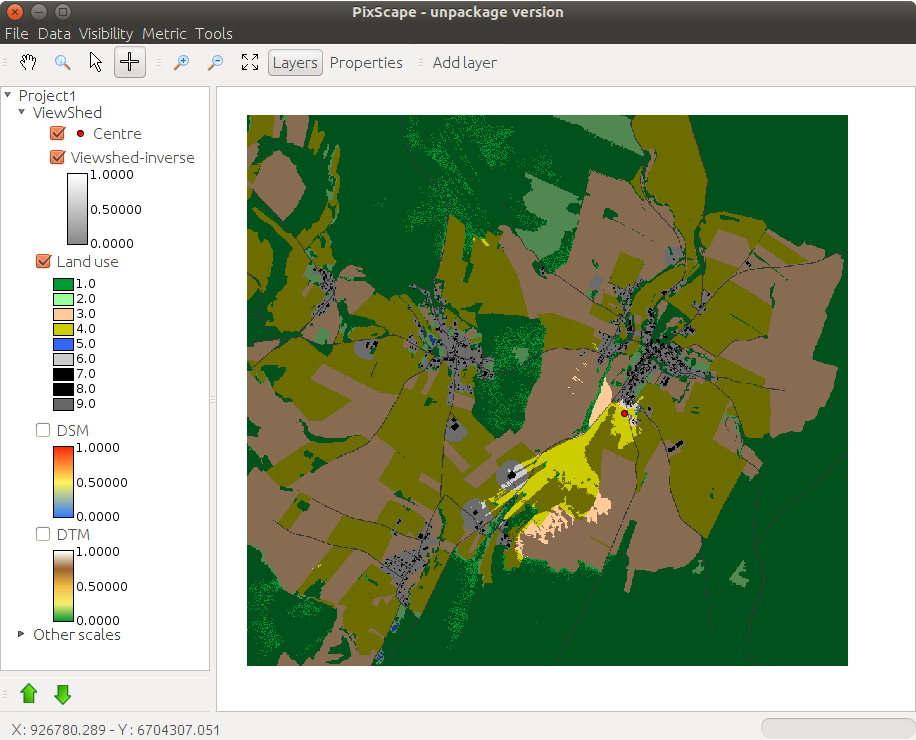
\includegraphics[scale=0.5]{img/viewshed-en.png} 
	\caption{Resulting viewshed from the red point. The viewshed is displayed by transparency.}
	\label{viewshed}
\end{figure}

The calculation of a viewshed can be accessed from the Visibility / Viewshed menu. A window appears showing all the parameters that are relevant for the calculation of a viewshed (figure \ref{viewshed_param_fig}).

\begin{figure}[H]
	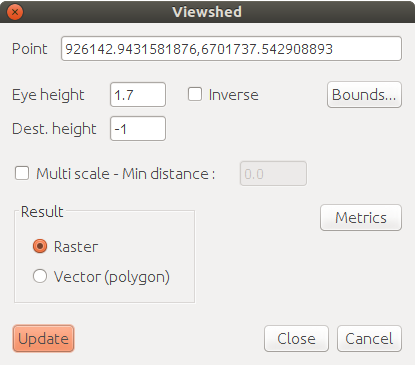
\includegraphics[scale=0.5]{img/viewshed_dlg-en.png} 
	\caption{Viewshed settings window}
	\label{viewshed_param_fig}
\end{figure}

\subsubsection{Parameters}
\label{viewshed_param}
\begin{itemize}
	\item Point: coordinates of the observation or observed point O. It can be entered manually or given by clicking on the map.
	\item Eye height (h1): height in meter of the observer eye
	\item Dest. height (h2): height in meters of observed point(s). If set to -1, the height of the DSM is used. If the project does not contain a DSM, the height is zero.
	\item Inverse: unchecked by default, point O is the observation point \textit{ie.} the eye of the observer (figure \ref{height_view}). The viewshed corresponds to all the points visible from O. Conversely, if the box is checked, the point O becomes the observed point (figure \ref{height_view_inverse}). The viewshed then corresponds to the set of points from which the observer sees the point O.
	\item Bounds: this window allows you to restrict the eyesight of the observer in the 3 dimensions (see \nameref{bounds})
	\item Multiscale: enables or disables multiscale calculation. If enabled, the minimal distance in meter before the change of scale must be entered.
\end{itemize}


\begin{figure}[H]
	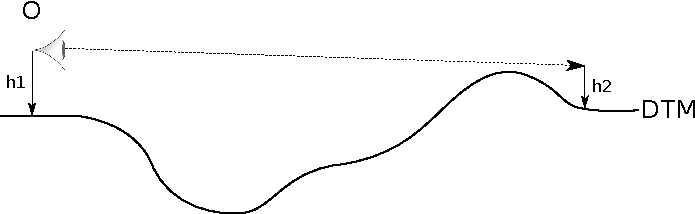
\includegraphics{img/height_view-en.pdf} 
	\caption{Default mode: O is the observation point, h1 is the height of the eye and h2 is the destination height or the DSM height if Dest. height = -1}
	\label{height_view}
\end{figure}

Dest. height (h2) parameter is often used with inverse mode to analyze the impact of a construction (pylon, wind turbine, etc). The resulting viewshed then corresponds to the set of points from which the new construction of a height h2 will be visible (figure \ref{height_view_inverse}).

\begin{figure}[H]
	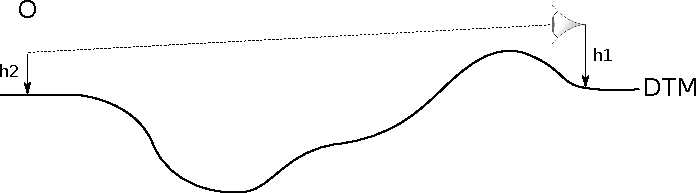
\includegraphics{img/height_view_inverse-en.pdf} 
	\caption{Inverse mode: O is the observed point, h1 is the height of the eye and h2 is the destination height (defined by  Dest. height or the DSM height if Dest. height = -1)}
	\label{height_view_inverse}	
\end{figure}

\subsubsection{Results}

The viewshed can be displayed on the map in raster or vector form according to the choice made in the Result panel. In raster, the bright areas correspond to the visible areas. Conversely, in vectorial, the dark areas correspond to the visible areas. In both cases, the result layer can be exported by right clicking on the layer.

Metrics can be selected from the Metrics button to be calculated on the current viewshed. For more information on metrics, see the section \nameref{metrics}.

\begin{figure}[H]
	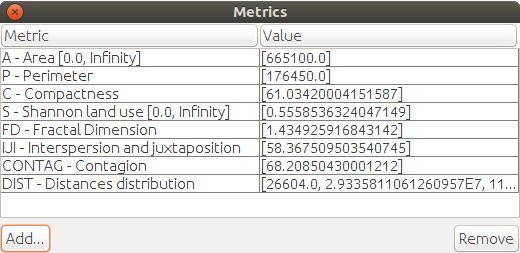
\includegraphics[scale=0.5]{img/viewshed_metric-en.png} 
	\caption{Metrics calculated from the current viewshed}
	\label{viewshed_metric}
\end{figure}

After modifying a parameter, simply click on the Update button to update the viewshed on the map as well as the metrics if they are displayed.


\subsection{Tangential view}

The calculation of a tangential view can be accessed from the Visibility / Tangential View menu. A window appears showing the settings for the calculation of the view as well as for displaying the result (figure \ref{viewtan_param}). 

\begin{figure}[H]
	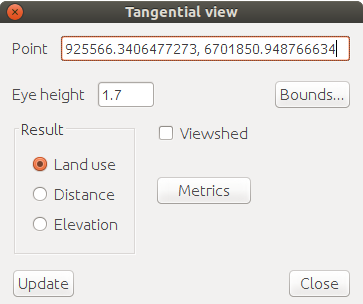
\includegraphics[scale=0.5]{img/viewtan_dlg-en.png} 
	\caption{Tangential view settings}
	\label{viewtan_param}
\end{figure}

\subsubsection{Parameters}

\begin{itemize}
	\item Point: coordinates of the observation or observed point O. It can be entered manually or given by clicking on the map.
	\item Eye height (h1): height in meter of the observer eye
	\item Bounds: this window allows you to restrict the eyesight of the observer in the 3 dimensions (see \nameref{bounds})
	\item Viewshed: if checked, the viewshed is displayed on the map.
	\item Result: choice of the result displayed (see \nameref{viewtan_result}).
\end{itemize}

The angular resolution parameter and the use of the multiscale database cannot be set in this window but only on the Options window (see \nameref{options}).

\subsubsection{Results}
\label{viewtan_result}
The result is displayed in a new window representing the tangential view (figure \ref{viewtan_land}). The coordinates of this image are in degrees from -180° to + 180° horizontally and -90° to + 90° vertically, the north being at 0° in the middle of the image.

\begin{figure}[H]
	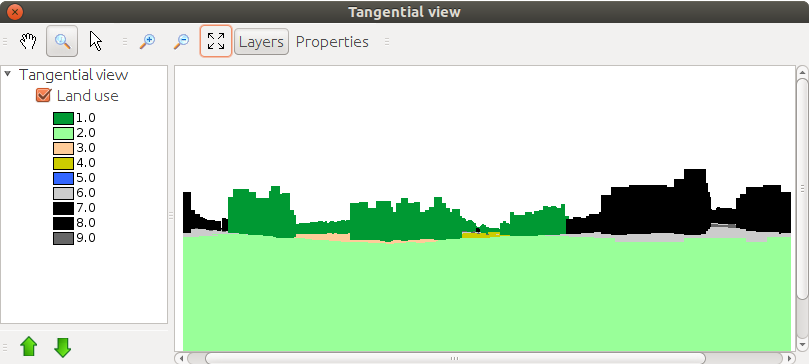
\includegraphics[scale=0.5]{img/viewtan_land-en.png} 
	\caption{Tangential view. The colors represent the land use.}
	\label{viewtan_land}
\end{figure}

By default, colors represent the land use categories (figure \ref{viewtan_land}). By selecting Distance in the result panel, the tangential view displays the distances to the observation point (figure \ref{viewtan_dist}).

\begin{figure}[H]
	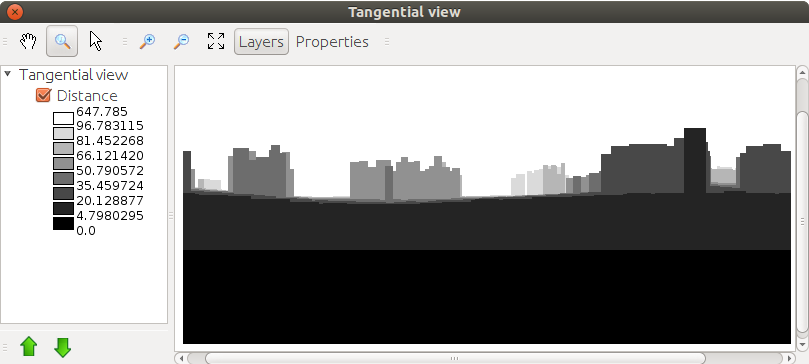
\includegraphics[scale=0.5]{img/viewtan_dist-en.png} 
	\caption{Tangential view. The colors represent the distance to the observation point.}
	\label{viewtan_dist}
\end{figure}

Metrics can be selected from the Metrics button to be calculated on the current view. For more information on metrics, see the section \nameref{metrics}.

After modifying a parameter, simply click on the Update button to update the view as well as the metrics if they are displayed.


\subsection{Multi-viewshed}
\label{multi_viewshed}
The Visibility / Multi Viewshed menu allows you to calculate several viewsheds from a shapefile containing observation points.

\begin{figure}[H]
	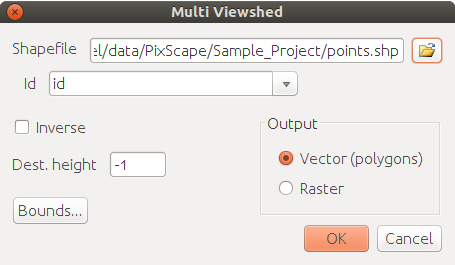
\includegraphics[scale=0.5]{img/multi_viewshed-en.png} 
	\caption{Multi-viewshed settings}
	\label{multi_viewshed_dlg}
\end{figure}

\subsubsection{Parameters}

\begin{itemize}
	\item Shapefile : shapefile containing observation points.
	\item Id : shapefile attribute used as identifier. This parameter is useful only for vectorial result.
	\item Inverse: unchecked by default, the shapefile points represent the observation points \textit{ie.} the eye of the observer. Conversely, if the box is checked, the shapefile points becomes the observed points. For details see the viewshed \nameref{viewshed_param}.
	\item Dest. height (h2): height in meters of observed point(s). If set to -1, the height of the DSM is used. If the project does not contain a DSM, the height is zero.
	\item Bounds: this window allows you to restrict the eyesight of the observer in the 3 dimensions for all observation points (see \nameref{bounds}). If the shapefile contains the attributes (dmin, dmax, zmin, zmax, orien et amp), they will be used in place of these settings.
	\item Output : format of the result layer : vector or raster.
\end{itemize}

The eye height (h1) parameter and the use of the multiscale database cannot be set in this window but only on the Options window (see \nameref{options}).

\subsubsection{Result}
The resulting viewsheds can be displayed on the map in raster or vector format according to the selected option on Output panel. In both cases, the result layer can be exported by right clicking on it.

In vector, the layer contains a multi-polygon for each viewshed (figure \ref{multi_viewshed_vector}). Each multi-polygon has an Id attribute allowing to link the shape with the corresponding observation point.

\begin{figure}[H]
	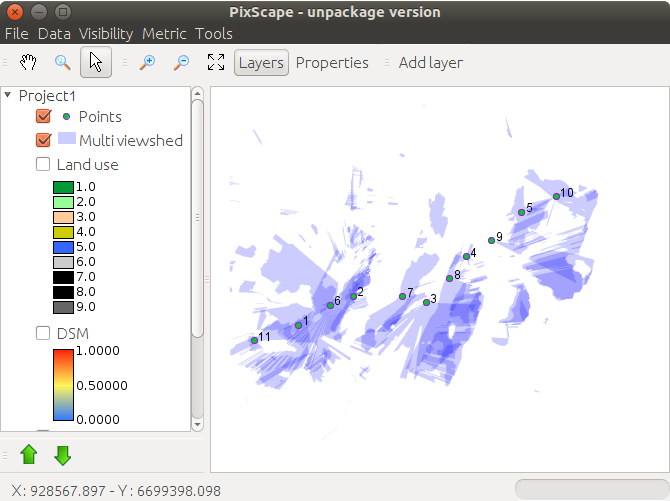
\includegraphics[scale=0.5]{img/multi_viewshed_vector-en.png} 
	\caption{Multi-viewshed in vector format}
	\label{multi_viewshed_vector}
\end{figure}

In raster, the value of the pixel corresponds to the number of times the pixel is contained in a viewshed \textit{ie.} the number of observation points seeing the pixel or, in inverse mode, the number of observation points seen from the pixel (figure \ref{multi_viewshed_raster}).

\begin{figure}[H]
	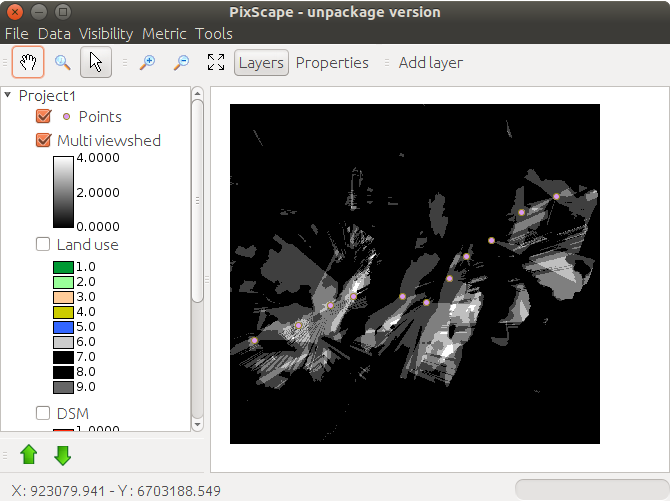
\includegraphics[scale=0.5]{img/multi_viewshed_raster-en.png} 
	\caption{Multi-viewshed in raster format}
	\label{multi_viewshed_raster}
\end{figure}

\subsection{Eyesight bounds}
\label{bounds_ui}
For all visibility calculations into PixScape, the eyesight can be restricted in all 3 dimensions. Details are described in the section \nameref{bounds}.

These bounds can be set from the Bounds window (figure \ref{bounds_dlg}). When the observation points come from a shapefile, the setting of the eyesight can be differentiated for each point by adding the 6 parameters (dmin, dmax, zmin, zmax, orien, amp) in the shapefile attributes table. The "Set point attributes" menu allows you to automatically add them to an existing shapefile (see \nameref{add_attributes}).

\begin{figure}[H]
	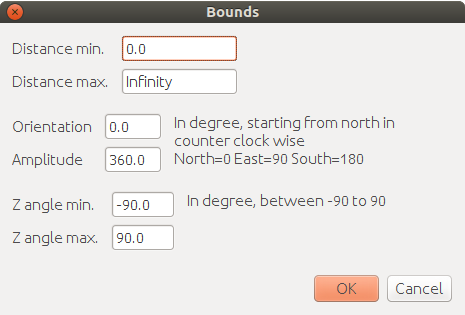
\includegraphics[scale=0.5]{img/bounds-en.png} 
	\caption{Settings of the eyesight. By default the eyesight bounds are unlimited.}
	\label{bounds_dlg}
\end{figure}

\section{Visibility metric calculation}
\label{calc_metrics}
PixScape can agregate the result of a viewshed or tangential view by several indicators, or metrics. The available metrics are detailed in the chapter \nameref{metrics}.

The Visibility menu already allows you to calculate several metrics on the current view. But this "manual" operation is only possible for a few observation points.

The Metric menu allows you to launch a visibility calculation (planimetric or tangential) and the calculation of the metrics for a set of observation points in a single execution.


\begin{figure}[H]
	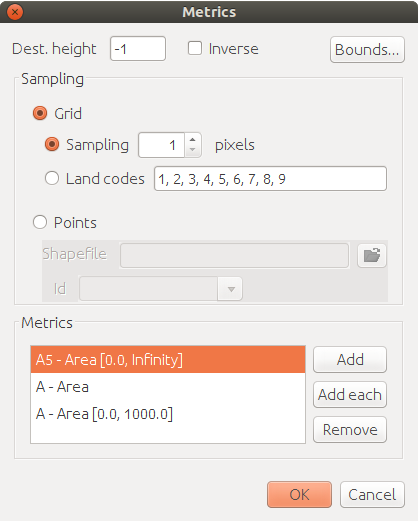
\includegraphics[scale=0.5]{img/metrics-en.png} 
	\caption{Settings for metrics calculation}
	\label{metrics_dlg}
\end{figure}

\subsection{View parameters}
View-specific parameters are displayed at the top of the window (figure \ref{metrics_dlg}) and depend on the type of view selected in the Metric menu: planimetric (for viewshed) or tangential.

\begin{itemize}
	\item Inverse (planimetric only): unchecked by default, the shapefile points represent the observation points \textit{ie.} the eye of the observer. Conversely, if the box is checked, the shapefile points becomes the observed points. For details see the viewshed \nameref{viewshed_param}.
	\item Dest. height (h2) (planimetric only): height in meters of observed point(s). If set to -1, the height of the DSM is used. If the project does not contain a DSM, the height is zero.
	\item Bounds: this window allows you to restrict the eyesight of the observer in the 3 dimensions for all observation points (see \nameref{bounds}). If the selected sampling is Points and the shapefile contains the attributes (dmin, dmax, zmin, zmax, orien et amp), they will be used in place of these settings.	
\end{itemize}

The other parameters for the view (\textit {eg.} eye height, angular resolution, ...) must be set before in the Options window (see \nameref{options}).


\subsection{Sampling}
\label{sampling}
Observation points can be given in raster (Grid option) or vector (Points option). The format of the result (raster or vector) is related to the type chosen.

\subsubsection{Grid sampling (raster)}
With grid option, the sampling of the observation points is done from the grid of the DTM at the finest resolution. Two options are possible: regular sampling on the grid or land use category.

By default, the sampling is regular and set at 1 pixel, which corresponds to an exhaustive run of the set of pixels of the image \textit{ie.} a visibility calculation will be executed from each pixel. If we increase the sampling to 3, only one pixel out of 3 will be used in each dimension, so we will compute a view only for 1 pixel out of 9 of the grid (figure \ref{grid_sampling}).

\begin{figure}[H]
	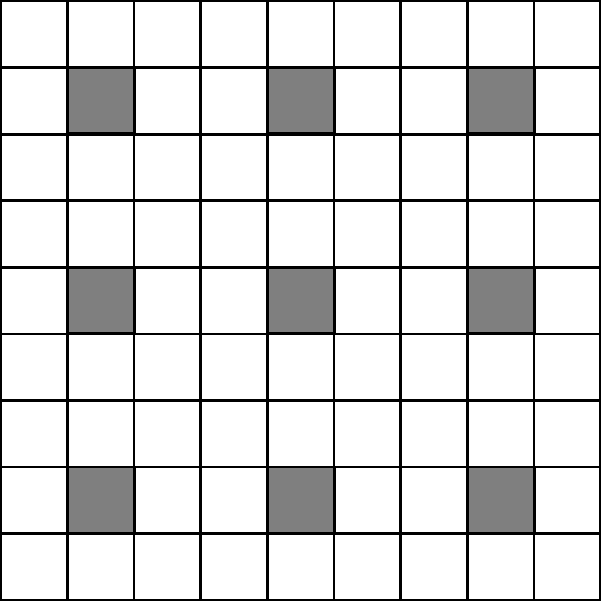
\includegraphics[scale=0.5]{img/grid_sampling.pdf} 
	\caption{Grid sampling every 3 pixels on each dimension. 9 views will be calculated from the 9 shaded pixels.}
	\label{grid_sampling}
\end{figure}

If the sampling is done by land use category, the views will be calculated only from the pixels belonging to one of the listed categories. Land use codes must be separated by commas.

The result will be one or more raster layers. It will contain one layer for each metric and for each distance range defined in the metric setting.


\subsubsection{Points sampling (vector)}
Instead of using the raster grid sampling, you can provide a set of points from a shapefile.

The result will be in the form of a point layer corresponding to the input shapefile. The result of the metrics will be stored in the attribute table of the shapefile.


\subsection{Metric parameters}
\label{param_metrics}
For each observation point, a set of metrics can be computed. The Metrics panel allows you to select them and to set distances and landuse categories if needed. The same metric can be added several times with different settings.

\begin{figure}[H]
	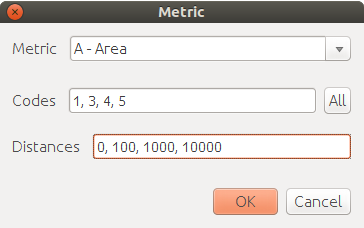
\includegraphics[scale=0.5]{img/metric_param-en.png} 
	\caption{Parameters of metric A}
	\label{metric_param_dlg}
\end{figure}

Figure \ref{metric_param_dlg} shows the settings of the metric A. In this example, metric A will only be calculated on the landuse classes 1, 3, 4 and 5 for 3 distance intervals [0-100[ , [100-1000[ and [1000-10000[. The result will contain 3 values for each observation point, one for each distance interval.

"Add each" button adds the selected metric several times: one for each land-use category.

Several landuse categories can be grouped in one class with the dash character "-" (figure \ref{metric_param_group_dlg}). This makes it possible to keep a detailed land-use and at the same time carry out some analysis on more general classes.

\begin{figure}[H]
	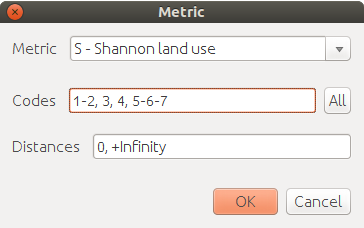
\includegraphics[scale=0.5]{img/metric_param_group-en.png} 
	\caption{Parameters of metric S. Land-use category are grouped in 4 classes.}
	\label{metric_param_group_dlg}
\end{figure}

The grouping of land-use categories is not useful for metric A. Indeed, this metric does not differentiate the categories in each class. For example, \verb|1,3,4,5| and \verb|1-3,4-5| will give the same result for the metric A.

\subsection{Results}

The result of the calculation of metrics is displayed on the map by one or more layers in raster or vector format depending on the input format used for sampling. Each layer can be exported by right clicking on the layer name and the "Export ..." menu.

\subsubsection{Raster}
For raster, the result is a set of raster layers, one for each metric and each distance interval. Each layer can be exported in Tiff or AsciiGrid format.

For the settings of the figure \ref{metric_param_dlg}, PixScape adds 3 raster layers (figure \ref{metric_result_rast}) for the 3 distance intervals.

If the sampling is greater than 1, the pixel size is increased proportionately as the sampling factor. 

\begin{figure}[H]
	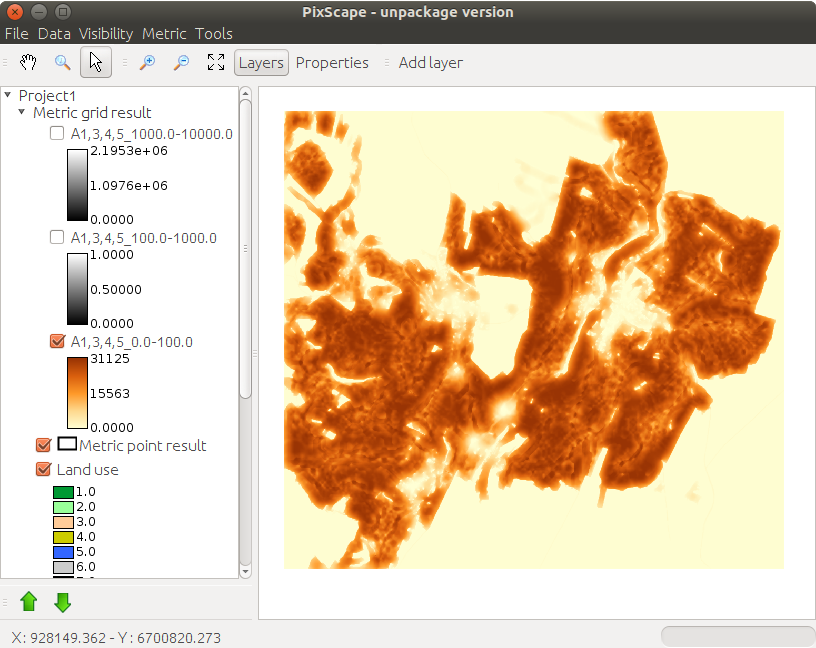
\includegraphics[scale=0.5]{img/metric_result_rast-en.png} 
	\caption{Metric result with grid sampling.}
	\label{metric_result_rast}
\end{figure}

\subsubsection{Vector}

In vector, the result is a point layer containing the metrics values in the attribute table (figure \ref{metric_result_attr}). By default the first metric is displayed with proportional circle (figure \ref{metric_result_vect}). To display another metric, simply change the attribute selected in the "Circle" tab of the layer style window.

\begin{figure}[H]
	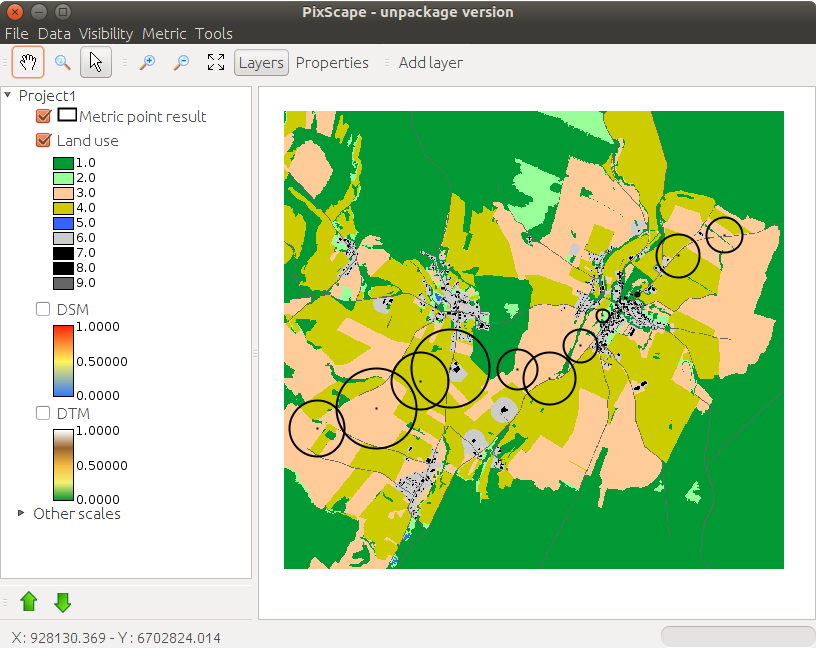
\includegraphics[scale=0.5]{img/metric_result_vect-en.png} 
	\caption{Metric result from a point layer. The first metric is displayed by circles proportional to the value of the metric.}
	\label{metric_result_vect}
\end{figure}

The layer "Metric point result" can be exported in shapefile or text format by right clicking on the layers name and the menu "Export ...".

\begin{figure}[H]
	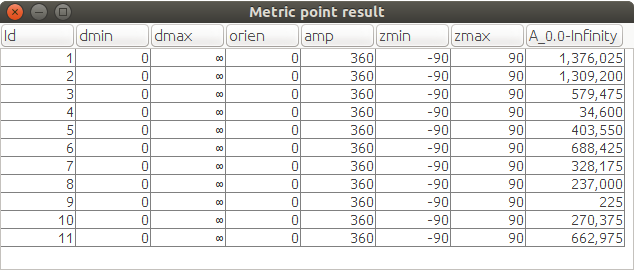
\includegraphics[scale=0.5]{img/metric_result_attr-en.png} 
	\caption{Attribute layer of the result layer.}
	\label{metric_result_attr}
\end{figure}

The attribute table of the result layer is accessible by right clicking on the layer name and the "Attribute table" menu. It contains, in addition to the metrics, the 6 parameters used for limiting the eyesight, allowing to keep these parameters with the results.

\section{Tools and options}
\label{tools}

\subsection{Add eyesight attributes}
\label{add_attributes}
For all visibility calculations, the eyesight can be restricted by the Bounds window (figure \ref{bounds_dlg}). This solution is useful if each observation point has the same limitations of the eyesight.
The Tools / Set point attributes menu is useful for specifying different restrictions for each observation point. This function adds the 6 attributes to a shapefile with the default values defined by the Bounds window. You can then with your favorite GIS modify the restriction values for each observation point.
The output shapefile can be used for calculation of metrics (\ref{calc_metrics}) or multi viewshed (\ref{multi_viewshed}).

\begin{figure}[H]
	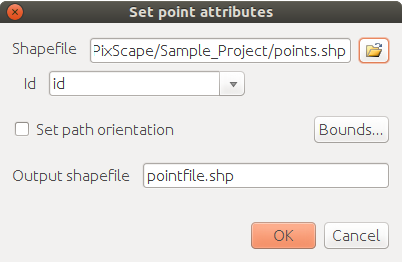
\includegraphics[scale=0.5]{img/add_attributes-en.png} 
	\caption{Add eyesight bound attributes to a shapefile}
	\label{add_attributes_dlg}
\end{figure}

\subsubsection{Eyesight along a path}
La case à cocher "Définir l'orientation selon le parcours" calcule l'orientation de chaque point par rapport au suivant. Avec cette option, le paramètre orientation de la fenêtre Limites sera ignoré et chaque point aura potentiellement une valeur d'orientation différente. 

\begin{figure}[H]
	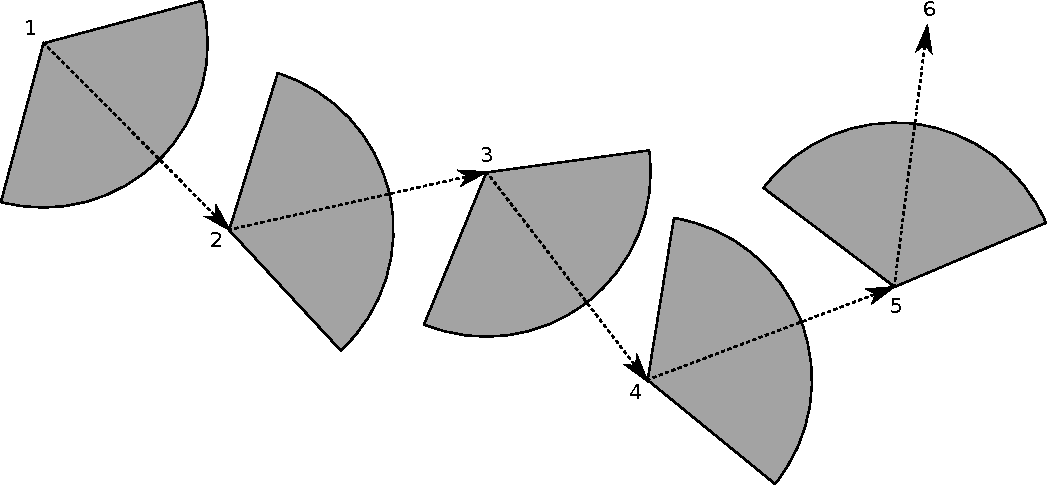
\includegraphics[scale=0.8]{img/path_orien.pdf} 
	\caption{Champ de vision le long d'un parcours. L'orientation est calculée en direction du point suivant et l'amplitude est constante.}
	\label{path_orien}
\end{figure}

L'ordre des points est défini par l'attribut id qui est trié par ordre croissant.
Cette option est utile uniquement avec une amplitude inférieure à 360°.


\subsection{Options}
\label{options}
Les options générales du projet sont accessibles à partir du menu Outils / Options.
Ces options sont enregistrées automatiquement dans le fichier xml du projet. Elles sont utilisées pour l'ensemble des calculs de visibilité sauf quand l'option est aussi présente dans la fenêtre de paramétrage d'un traitement. Par exemple, la hauteur de l'oeil est modifiable directement dans la fenêtre de paramétrage d'une vue planimétrique ou tangentielle, mais elle ne l'est pas pour le calcul des métriques. Dans ce dernier cas, la hauteur de l'oeil de l'observateur sera celle définie dans la fenêtre d'options.

\begin{figure}[H]
	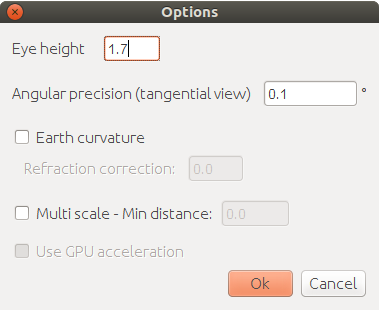
\includegraphics[scale=0.5]{img/options-en.png} 
	\caption{Options générales}
\end{figure}

\subsubsection{Hauteur de l'oeil de l'observateur}
Le paramètre Hauteur oeil ($h1$) spécifie la hauteur de l'observateur à partir du MNT. L'unité est le mètre. Pour plus de détails, voir \nameref{principles} et la figure \ref{ray_side}.

\subsubsection{Précision angulaire}
Le paramètre Précision angulaire ($\alpha$) définit la résolution en degré de la vue tangentielle. Il est fixé par défaut à 0.1°, ce qui correspond à 3600 rayons calculés si l'amplitude de la vue est à 360°. Pour plus de détails, voir \nameref{principles_tan} et la figure \ref{grid_tan}. 

\subsubsection{Courbure terrestre}
\label{curvature}
Les calculs de visibilité dans PixScape peuvent tenir compte de la courbure de la Terre, susceptible de jouer un rôle dans le cas d'une vue à plusieurs dizaines de kilomètres. Le principe du calcul est simple : plus la distance à l'observateur augmente, plus la hauteur des objets visibles diminuent. 
La hauteur tenant compte de la courbure de la Terre $z'_i$ d'un point $i$ est calculée comme suit : 

$$z'_i = z_i - \frac{d_i^2}{D}$$

avec $z_i$ l'altitude du MNT au point $i$, $d_i$ la distance entre le point $i$ et l'observateur et $D$ le diamètre de la Terre (12 740 000 mètres).

La courbure de la Terre peut être compensée en partie par la réfraction de la lumière dans l'atmosphère. Dans PixScape, à partir du moment où la courbure terrestre est prise en compte, le paramètre de réfraction peut être spécifié. Il est défini par défaut à 0,13. Le calcul de la hauteur devient : 

$$z'_i = z_i - (1-\rho)\frac{d_i^2}{D}$$

avec $\rho$ le coefficient de réfraction compris entre 0 et 1. Si $\rho=0$ on retombe sur la formule précédente sans réfraction.


\subsubsection{Multi-résolution}
A partir du moment où le projet contient les données à plusieurs résolutions, les calculs de visibilité peuvent se faire en multi-résolution en activant cette option. Le paramètre de distance minimale est à définir obligatoirement. Il permet d'assurer une distance minimale en mètre avant de changer de résolution. 

Pour plus de détails sur le calcul de visibilité en multi-résolution, voir \nameref{multires}.


\subsubsection{Accélération GPU}
Ce paramètre permet de réaliser les calculs de visibilité sur la carte graphique au lieu du processeur. Les gains en temps d'exécution peuvent être importants pour des cartes graphiques Nvidia de la gamme Tesla, conçues pour le calcul haute performance (voir \nameref{perf}). En revanche, toutes les métriques ne sont pas optimisées pour le GPU. Les métriques A et S sont les seules à être optimisées. Si vous utilisez d'autres métriques, les gains de temps seront minimes voire inexistants.

Le paramètre est grisé si PixScape ne peux pas utiliser l'accélération GPU. Les causes peuvent être multiples : pas de carte graphique NVidia, pas de support de CUDA, pas la bonne version de CUDA (6.5).

Si l'option multi-résolution est active, l'accélération GPU ne sera pas utilisée même si elle est activée.


\chapter{Interface en ligne de commande}
\label{cli}

Dès lors qu'un projet a été créé depuis l'interface graphique, il est possible d'utiliser PixScape en ligne de commande. Ce mode est utile pour exécuter le logiciel sur un ordinateur distant sans interface graphique, lancer automatiquement plusieurs traitements à la suite, ou encore soumettre des exécutions sur un cluster.

\section{Démarrage}

\subsection{Lancer PixScape en ligne de commande}
Il faut tout d'abord ouvrir une fenêtre de terminal, puis aller dans le répertoire contenant PixScape avec la commande \textit{cd}.
Enfin, vous pouvez saisir la commande suivante pour afficher l'écran d'aide de PixScape :
\begin{Verbatim}
java -jar pixscape.jar --help
\end{Verbatim}
Résultat
\begin{Verbatim}
Usage :
java -jar pixscape.jar --metrics
...
...
\end{Verbatim}
Vous êtes prêt à utiliser PixScape en ligne de commande.

\subsection{Syntaxe}
\subsubsection{Définition}
Les commandes commencent par un double tiret : \verb|--project, --metrics, ...|\\
Les options globales commencent par un tiret simple : \verb|-proc, -bounds, ...|\\
Les paramètres n'ont pas de tiret : \verb|dmin, inverse, ...|

\subsubsection{Séparateur}
Les espaces sont utilisés pour séparer les différents éléments d'une ligne de commande, par conséquent, vous ne pouvez pas avoir un nom qui contient des espaces.\\

\subsubsection{Syntaxe de l'écran d'aide}
Dans l'écran d'aide, les éléments entourés de crochets sont optionnels, et donc les éléments qui ne sont pas entourés par des crochets sont obligatoires. Le caractère \verb+|+ sépare les options possibles.

\section{Commandes}

\subsection{--help : affichage de l'aide}
Commande :
\begin{Verbatim}
java -jar pixscape-1.0.jar --help
\end{Verbatim}
Résultat :
\begin{Verbatim}
Usage :
java -jar pixscape.jar --metrics
java -jar pixscape.jar [-mpi | -proc n | -cuda n]
--project project_file.xml
[--landmod zone=filezones.shp id=fieldname code=fieldname dsm=file.tif [selid=id1,...,idn]]
[-zeye val] [-zdest val] [-resdir path]
[-bounds [dmin=val] [dmax=val] [orien=val] [amp=val] [zmin=val] [zmax=val]]
[-sampling n=val | land=code1,..,coden | points=pointfile.shp id=fieldname]
[-multi dmin=val | -mono]
[-earth flat|curved [refrac=val]]
commands

Commands list :
--viewshed [inverse] x y [resfile=raster.tif]
--viewtan [prec=deg] x y [resname=name]
--planmetric [inverse] metric1[[code1,...,coden]][_d1,...,dm] ... metricn[[code1,...,coden]][_d1,...,dm]
--tanmetric [prec=deg] metric1[[code1,...,coden]][_d1,...,dm] ... metricn[[code1,...,coden]][_d1,...,dm]
\end{Verbatim}

\subsection{--metrics : affichage des métriques}
Cette commande affiche l'ensemble des métriques disponibles avec leur abréviation et leur nom. 

Commande :
\begin{Verbatim}
java -jar pixscape-1.0.jar --metrics
\end{Verbatim}
Résultat :
\begin{Verbatim}
===== Metrics =====
A - Surface
P - Périmètre
C - Compacité
S - Shannon OS
FD - Dimension fractale
IJI - Interspersion et juxtaposition
CONTAG - Contagion
DIST - Distribution des distances
SL - Ligne d'horizon
SD - Shannon distances max.
DL - Profondeur de vue
\end{Verbatim}

\subsection{--project : chargement d'un projet}
Cette commande définit le chemin vers le fichier xml du projet à charger.
\begin{Verbatim}[commandchars=\\\{\}]
java -jar pixscape-1.0.jar --project \textit{path2myproject/myproject.xml}
\end{Verbatim}
Charge le projet \textit{myproject} contenu dans le répertoire \textit{path2myproject}.

La commande \verb|--project| ne peut être utilisée qu'une seule fois et doit être la première commande de la ligne.
Toutes les commandes qui suivent dans ce manuel ont besoin d'un projet chargé.

\subsection{--landmod : changements d'occupation du sol}

\begin{Verbatim}[commandchars=\\\{\}]
--landmod zone=\textit{filezones.shp} id=\textit{fieldname} code=\textit{fieldname} dsm=\textit{file.tif} [selid=\textit{id1,...,idn}]
\end{Verbatim}

\subsubsection{Paramètres obligatoires}
\begin{itemize}
	\item \verb|zone=filezones.shp| : shapefile de polygones contenant les changements d'occupation du sol
	\item \verb|id=fieldname| : nom d'un attribut du shapefile servant à identifier les polygones. Si les valeurs ne sont pas uniques, les polygones ayant le même identifiant seront appliqués en un seul changement.
	\item \verb|code=fieldname| : nom d'un attribut du shapefile stockant la nouvelle catégorie d'occupation du sol du polygone
	\item \verb|dsm=file.tif| : raster stockant les nouvelles valeurs de MNE utilisées à chaque changement d'occupation du sol. La géométrie du raster doit être exactement la même que le MNT du projet.
\end{itemize}

\subsubsection{Paramètre optionnel}
\begin{itemize}
	\item \verb|selid=id1,...,idn| : liste des identifiants de polygones à traiter. Si ce paramètre n'est pas renseigné tous les polygones du shapefile sont utilisés.
\end{itemize}

\subsubsection{Description}
Cette commande doit être placée avant les commandes de calcul de visibilité. Elle va dupliquer le projet pour chaque polygone du shapefile et modifier l'occupation du sol couvert par le polygone ainsi que le MNE. Les commandes suivantes seront exécutées sur chaque projet modifié.

Les projets créés seront nommés par l'identifiant du (ou des) polygones et stockés dans le répertoire du projet.

\subsection{--viewshed : vue planimétrique}
\begin{Verbatim}[commandchars=\\\{\}]
--viewshed [inverse] \textit{x} \textit{y} [resfile=\textit{raster.tif}]
\end{Verbatim}

\subsubsection{Paramètres obligatoires}
\begin{itemize}
	\item \verb|x| : abscisse du point d'observation dans le système de coordonnées du MNT
	\item \verb|y| : ordonnée du point d'observation dans le système de coordonnées du MNT
\end{itemize}

\subsubsection{Paramètres optionnels}
\begin{itemize}
	\item \verb|inverse| : passe en mode inverse, le point O devient le point observé
	\item \verb|resfile=raster.tif| : permet de spécifier un autre nom pour le fichier stockant le résultat
\end{itemize}

\subsubsection{Description}
La commande \verb|--viewshed| permet de calculer le bassin de visibilité à partir d'un point d'observation. Le résultat est stocké dans un fichier raster de la même taille que le MNT, au format Tiff. Dans ce raster, le bassin de visibilité est formé des pixels dont la valeur est à 1, les autres sont à 0.

\subsubsection{Exemples}
L'exemple ci-dessous calcule le bassin de visibilité pour un observateur situé au point de coordonnées (925560, 6702495). Le résultat sera stocké dans le répertoire du projet dans un fichier nommé : \verb|viewshed-925560,6702495.tif|.
\begin{Verbatim}
	--viewshed 925560 6702495
\end{Verbatim}

Le second exemple calcule le bassin de visibilité en mode inverse et enregistre le résultat dans le fichier \verb|bassin1.tif|.
\begin{Verbatim}
	--viewshed inverse 925560 6702495 resfile=bassin1.tif
\end{Verbatim}

\subsection{--viewtan : vue tangentielle}
\begin{Verbatim}[commandchars=\\\{\}]
--viewtan [prec=\textit{deg}] \textit{x} \textit{y} [resname=\textit{name}]
\end{Verbatim}

\subsubsection{Paramètres obligatoires}
\begin{itemize}
	\item \verb|x| : abscisse du point d'observation dans le système de coordonnées du MNT
	\item \verb|y| : ordonnée du point d'observation dans le système de coordonnées du MNT
\end{itemize}

\subsubsection{Paramètres optionnels}
\begin{itemize}
	\item \verb|prec=deg| : défini la précision angulaire en degré. Si ce paramètre n'est pas défini, la précision angulaire enregistrée dans le projet sera utilisée.
	\item \verb|resname=name| : permet de spécifier un autre nom pour les fichiers stockant le résultat
\end{itemize}

\subsubsection{Description}
La commande \verb|--viewtan| permet de calculer la vue tangentielle à partir d'un point d'observation. Les résultats sont stockés dans 2 ou 3 fichiers rasters au format Tiff selon si le projet contient une couche d'occupation du sol. 
\begin{itemize}
	\item \verb|elev| : altitude du MNT
	\item \verb|dist| : distance 2D au point d'observation
	\item \verb|land| : occupation du sol, si présent dans le projet
\end{itemize}

La taille des raster dépend de la précision angulaire. Pour une précision de 0,1° et une vue à 360°, les images auront une taille de 3600x1800 pixels. Leur système de coordonnées est défini en degré. 

\subsubsection{Exemples}
L'exemple ci-dessous calcule la vue tangentielle pour un observateur situé au point de coordonnées (925560, 6702495). Le résultat sera stocké dans le répertoire du projet dans les fichiers nommés : \verb|viewshed-925560,6702495-elev.tif|, \verb|viewshed-925560,6702495-dist.tif| et \verb|viewshed-925560,6702495-land.tif| si le projet contient une couche d'occupation du sol.
\begin{Verbatim}
	--viewtan 925560 6702495
\end{Verbatim}

Le second exemple calcule la vue tangentielle avec une précision angulaire de 0,05° et enregistre le résultat dans les fichiers \verb|vue1-elev.tif|, \verb|vue1-dist.tif| et \verb|vue1-land.tif| si le projet contient une couche d'occupation du sol.
\begin{Verbatim}
	--viewshed prec=0.05 925560 6702495 resname=vue1
\end{Verbatim}


\subsection{--multiviewshed : bassin de visibilité multiple}
\begin{Verbatim}[commandchars=\\\{\}]
--multiviewshed format=vector|raster [inverse] [resname=\textit{name}]
\end{Verbatim}

\subsubsection{Paramètre obligatoire}
\begin{itemize}
	\item \verb/format=vector|raster/ : format du résultat (shapefile ou tiff)
\end{itemize}

\subsubsection{Paramètres optionnels}
\begin{itemize}
	\item \verb|inverse| : passe en mode inverse, le point O devient le point observé
	\item \verb|resname=name| : permet de spécifier un autre nom pour le fichier stockant le résultat
\end{itemize}

\subsubsection{Description}
La commande \verb|--multiviewshed| permet de calculer les bassins de visibilité à partir d'un ensemble de points d'observation. Les points d'observation doivent être donnés par l'option \verb|-sampling|. Le résultat est stocké dans un fichier raster ou vecteur selon le format choisi. 

En raster, l'image est de la même taille que le MNT, au format Tiff. Dans ce raster, chaque pixel recense le nombre de fois qu'il est vu depuis les points d'observation et en mode inverse le nombre de points vu à partir de ce pixel.

En vectoriel, le résultat est un shapefile contenant le bassin de visibilité de chaque point d'observation.

\subsubsection{Exemples}
L'exemple ci-dessous calcule les bassins de visibilité des points d'observation donnés dans le shapefile points.shp et stocke le résultat dans un shapefile dans le répertoire du projet nommé : \verb|multiviewshed.shp|.
\begin{Verbatim}
-sampling points=points.shp id=fid --multiviewshed format=vector
\end{Verbatim}



\subsection{--planmetric : métriques en vue planimétrique}

\begin{Verbatim}[commandchars=\\\{\}]
--planmetric [inverse] \textit{metric1}[[\textit{code1,...,coden}]][_\textit{d1,...,dm}] ...
\end{Verbatim}

\subsubsection{Paramètres obligatoires}
\begin{itemize}
	\item \verb|metric1[[code1,...,coden]][_d1,...,dm]| : métrique planimétrique à calculer avec ses paramètres (cf. \nameref{param_metrics_cli}).
	\item ...
\end{itemize}

\subsubsection{Paramètre optionnel}
\begin{itemize}
	\item \verb|inverse| : passe en mode inverse, les points d'observation deviennent les points observés
\end{itemize}

\subsubsection{Description}
La commande \verb|--planmetric| permet de calculer un ensemble de métriques en vue planimétrique. Les points d'observation sont définis en amont par l'option globale \verb|-sampling|. Si l'option n'est pas renseignée, l'échantillonnage par défaut se fait sur la grille pour tous les pixels du MNT ($n=1$).

Les résultats sont stockés dans plusieurs fichiers Tiff pour un échantillonnage sur la grille et dans un shapefile pour un échantillonnage vectoriel.


\subsubsection{Exemples}

L'exemple ci-dessous calcule la métrique A sans paramètre. Si l'échantillonnage est sur la grille, le résultat sera stocké dans le fichier \verb|A-.tif|.
\begin{Verbatim}
	--planmetric A
\end{Verbatim}

L'exemple ci-dessous calcule en vue inversée la métrique A pour le code d'occupation du sol 1 et la métrique A pour le code 2. Si l'échantillonnage est sur la grille, le résultat sera stocké dans les fichiers \verb|A1-.tif| et \verb|A2-.tif|.
\begin{Verbatim}
	--planmetric inverse A[1] A[2]
\end{Verbatim}


\subsection{--tanmetric : métriques en vue tangentielle}
\begin{Verbatim}[commandchars=\\\{\}]
--tanmetric [prec=\textit{deg}] \textit{metric1}[[\textit{code1,...,coden}]][_\textit{d1,...,dm}] ...
\end{Verbatim}

\subsubsection{Paramètres obligatoires}
\begin{itemize}
	\item \verb|metric1[[code1,...,coden]][_d1,...,dm]| : métrique tangentielle à calculer avec ses paramètres (cf. \nameref{param_metrics_cli}).
	\item ...
\end{itemize}

\subsubsection{Paramètre optionnel}
\begin{itemize}
	\item \verb|prec=deg| : précision angulaire en degrés
\end{itemize}

\subsubsection{Description}
La commande \verb|--tanmetric| permet de calculer un ensemble de métriques en vue tangentielle. Les points d'observation sont définis en amont par l'option globale \verb|-sampling|. Si l'option n'est pas renseignée, l'échantillonnage par défaut se fait sur la grille pour tous les pixels du MNT ($n=1$).

Les résultats sont stockés dans plusieurs fichiers Tiff pour un échantillonnage sur la grille et dans un shapefile pour un échantillonnage vectoriel.


\subsubsection{Exemples}

L'exemple ci-dessous calcule la métrique A sans paramètre. Si l'échantillonnage est sur la grille, le résultat sera stocké dans le fichier \verb|A-.tif|.
\begin{Verbatim}
	--tanmetric A
\end{Verbatim}

L'exemple ci-dessous calcule les vues tangentielles avec une précision angulaire de 0,05°. La métrique A est calculée 2 fois : pour le code d'occupation du sol 1 et pour le code 2. Si l'échantillonnage est sur la grille, le résultat sera stocké dans les fichiers \verb|A1-.tif| et \verb|A2-.tif|.
\begin{Verbatim}
	--tanmetric prec=0.05 A[1] A[2]
\end{Verbatim}


\section{Paramétrage des métriques}
\label{param_metrics_cli}
Le calcul des métriques peut être restreint à certaines catégories d'occupation du sol ou à certains intervalles de distance. Toutes les métriques ne supportent pas ces paramétrages. Pour connaitre quelle métrique supporte quel paramétrage, voir \nameref{metrics}.

\subsection{Occupation du sol}
Le calcul des métriques peut être restreint à certaines catégories d'occupation du sol en listant les catégories voulues entre crochet :
\begin{Verbatim}
	A[1,3,4,5]
\end{Verbatim}

Pour les métriques différenciant les catégories d'occupation du sol en classe (métriques S, IJI et CONTAG), les catégories peuvent être regroupées en une classe par le caractère \verb|-|. L'exemple ci-dessous regroupe les 6 catégories d'occupation du sol en 3 classes : 1-2-3, 4 et 5-6.
\begin{Verbatim}
	S[1-2-3,4,5-6]
\end{Verbatim}

\subsection{Distances}
Le calcul des métriques peut aussi être restreint à certains intervalles de distance avec le caractère \verb|_|. L'exemple ci-dessous calculera la métrique A pour 3 intervalles de distance : 0 à 100m, de 100 à 1000m et plus de 1000m. Il faut donc renseigner 4 distances pour obtenir 3 intervalles.
\begin{Verbatim}
	A_0,100,1000,+Infinity
\end{Verbatim}

Pour les métriques A et S, il est possible de restreindre par occupation du sol et par intervalle de distance. Dans ce cas de figure, les catégories d'occupation du sol doivent être données avant les distances :
\begin{Verbatim}
	A[1,2,3]_0,100,1000,+Infinity
\end{Verbatim}

\textbf{Dans tous les cas, il ne faut aucun espace dans la définition d'une métrique et de ses paramètres !}

\section{Options}

\subsection{Parallélisation : -mpi, -proc, -cuda}
\begin{Verbatim}[commandchars=\\\{\}]
-mpi | -proc \textit{n} | -cuda \textit{n}
\end{Verbatim}

PixScape supporte 3 modes de parallélisation en ligne de commande : par thread pour un ordinateur contenant plusieurs coeurs (\verb|-proc|), sur carte graphique (\verb|-cuda|) ou bien sur cluster (\verb|-mpi|).

Pour plus de détails voir la section \nameref{parallelism}.

Si aucune des 3 options n'est renseignée, la parallélisation par thread sera utilisée avec le nombre de coeurs défini dans l'interface graphique.

\subsection{Paramétrage de la vue : -zeye, -zdest, -bounds, -earth}

\subsubsection{-zeye}
\begin{Verbatim}[commandchars=\\\{\}]
-zeye \textit{val}
\end{Verbatim}
L'option \verb|-zeye| permet de définir la hauteur de l'oeil de l'observateur ($h1$). Si elle n'est pas renseignée, la hauteur de l'oeil enregistrée dans le projet sera utilisée à la place.

\subsubsection{-zdest}
\begin{Verbatim}[commandchars=\\\{\}]
-zdest \textit{val}
\end{Verbatim}
L'option \verb|-zdest| permet de définir la hauteur des pixels observés ($h2$). Si elle n'est pas définie, la hauteur du MNE est utilisée.

\subsubsection{-bounds}
\begin{Verbatim}[commandchars=\\\{\}]
-bounds [dmin=\textit{val}] [dmax=\textit{val}] [orien=\textit{val}] [amp=\textit{val}] [zmin=\textit{val}] [zmax=\textit{val}]
\end{Verbatim}
L'option \verb|-bounds| permet de restreindre le champ de vision dans les 3 dimensions par 6 paramètres : \verb|dmin|, \verb|dmax|, \verb|zmin|, \verb|zmax|, \verb|orien|, \verb|amp|. Pour plus de détails sur les paramètres, voir \nameref{bounds}.

\subsubsection{-earth}
\begin{Verbatim}[commandchars=\\\{\}]
-earth flat|curved [refrac=\textit{val}]
\end{Verbatim}

L'option \verb|-earth| permet de définir si la courbure de la Terre doit être pris en compte ou pas. Le paramètre \verb|flat| désactive le calcul de courbure et le paramètre \verb|curved| l'active. Dans ce dernier cas, le coefficient de réfraction de l'atmosphère peut être renseigné par le paramètre \verb|refrac|.

Pour plus de détails sur le calcul de la courbure, voir \nameref{curvature}.

Si cette option n'est pas renseignée, le paramétrage enregistré dans le projet sera utilisé à la place.

\subsection{Echantillonnage : -sampling}
\begin{Verbatim}[commandchars=\\\{\}]
-sampling n=\textit{val} | land=\textit{code1,..,coden} | points=\textit{pointfile.shp} id=\textit{fieldname}
\end{Verbatim}

L'échantillonnage définissant les points d'observation peuvent être donnés en raster ou en vectoriel. Pour plus de détails sur le fonctionnement de l'échantillonnage voir \nameref{sampling}.

L'option \verb|-sampling| est utilisée uniquement par les commandes \verb|--planmetric| et  \verb|--tanmetric|.

Si cette option n'est pas renseignée, l'échantillonnage exhaustif sur la grille sera utilisé : \verb|-sampling n=1|.

\subsubsection{Echantillonnage raster}
\begin{Verbatim}[commandchars=\\\{\}]
-sampling n=\textit{val} | land=\textit{code1,..,coden}
\end{Verbatim}
En raster, 2 échantillonnages sont possibles : régulier (\verb|n|) ou par catégorie d'occupation du sol (\verb|land|).


\subsubsection{Echantillonnage vectoriel}
\begin{Verbatim}[commandchars=\\\{\}]
-sampling points=\textit{pointfile.shp} id=\textit{fieldname}
\end{Verbatim}
Avec un échantillonnage issu d'un shapefile, le résultat des commandes \verb|--planmetric| et \verb|--tanmetric| est stocké dans un shapefile nommé \verb|metrics-pointfile.shp|.

Cette option est aussi utilisée par la commande \verb|--multiviewshed|.


\subsection{Multi-résolution : -multi, -mono}
\begin{Verbatim}[commandchars=\\\{\}]
-multi dmin=\textit{val} | -mono
\end{Verbatim}

Le calcul en multi-résolution peut être activé ou désactivé avec respectivement l'option \verb|-multi| et \verb|-mono|. 
L'option \verb|-multi| a besoin du paramètre \verb|distmin| pour définir la distance minimale avant de changer de résolution. Pour utiliser cette option, le projet doit contenir des données multi-résolution. 

Si aucune des 2 options n'est renseignée, le paramétrage enregistré dans le projet sera utilisé à la place.

\subsection{Emplacement des résultats : -resdir}
\begin{Verbatim}[commandchars=\\\{\}]
-resdir \textit{path}
\end{Verbatim}
Par défaut les résultats sont enregistrés dans le répertoire du projet. L'option \verb|-resdir| permet de modifier le répertoire par défaut. 
Si le répertoire donné n'existe pas, il sera créé automatiquement.

Si c'est un chemin relatif qui est donné, le chemin absolu sera déterminé à partir du répertoire courant au lancement de PixScape.

\section{Exemples}

Dans cette section, quelques exemples de lignes de commande complètes sont illustrés.

\subsection{Métriques tangentielles à partir d'un shapefile de points}
\subsubsection{Exemple simple}
\begin{Verbatim}
java -jar pixscape-1.0.jar --project Project1/Project1.xml 
	-sampling points=Points_IDF.shp id=Id 
	--tanmetric A SL DL
\end{Verbatim}

L'exemple ci-dessus, charge le projet \verb|Project1/Project1.xml| et calcule plusieurs métriques tangentielles (\verb|--tanmetric A SL DL|) à partir d'un ensemble de points d'observation défini dans le shapefile \verb|Points_IDF.shp|. Le résultat sera enregistré dans un shapefile nommé \verb|metrics-Points_IDF.shp|, contenant les points d'observations, et les valeurs des 3 métriques.

\subsubsection{Exemple complet}
\begin{Verbatim}
java -Xmx4g -jar  pixscape-1.0.jar -proc 8 --project Project1/Project1.xml -zeye 1.75
	-resdir res_tan -bounds zmin=-20 zmax=30 -sampling points=Points_IDF.shp 
	id=Id --tanmetric prec=0.01 A_0,100,1000,+Infinity A[5] A[6] SL DL
\end{Verbatim}

L'exemple suivant reprend la même base que le précédent mais avec plus de paramètres. Dans celui-ci la mémoire maximale allouée à PixScape est définie à 4 gigaoctets (\verb|-Xmx4g|) et le calcul est parallélisé sur 8 coeurs (\verb|-proc 8|). La hauteur de l'oeil de l'observateur est défini à 1,75 mètres (\verb|-zeye 1.75|). Les résultats ne seront pas enregistrés dans le dossier du projet mais dans un sous-dossier \verb|res_tan| (\verb|-resdir res_tan|). Le champ de vision est restreint dans l'angle vertical entre -20° et 30° (\verb|-bounds zmin=-20 zmax=30|). La précision angulaire est définie à 0,01° (\verb| prec=0.01|). Enfin la métrique A est décomposée d'une part pour 3 intervalles de distance (\verb|A_0,100,1000,+Infinity|) et pour 2 catégories d'occupation du sol (\verb|A[5] A[6]|).

\subsection{Métriques planimétriques à partir de la grille}
\begin{Verbatim}
java -jar  pixscape-1.0.jar -cuda 2 --project Project1/Project1.xml
	-resdir res_plan -sampling land=4 
	--planmetric A A[2,3] A[10] S
\end{Verbatim}
L'exemple ci-dessus, charge le projet \verb|Project1/Project1.xml| et calcule plusieurs métriques planimétriques (\verb|--planmetric A A[2,3] A[10] S|) à partir des points ayant la catégorie 4 d'occupation du sol (\verb|-sampling land=4|). Les résultats seront enregistrés dans le un sous-dossier du projet nommé \verb|res_plan|. Il contiendra 4 fichiers tiff : \verb|A-.tif|, \verb|A2,3-.tif|, \verb|A10-.tif| et \verb|S-.tif|. Enfin PixScape utilisera l'accélération GPU sur 2 cartes graphiques (\verb|-cuda 2|).


\chapter{Description des calculs de visibilité}
\label{principles}
Un calcul de visibilité se fait à partir d'un point d'observation noté O. A partir de ce point, un ensemble de rayons sont calculés pour déterminer les pixels visibles ou non. 
PixScape implémente deux méthodes de calcul de visibilité : la vue planimétrique représentant le bassin de visibilité sur le plan (x,y) et la vue tangentielle représentant la vue "réelle" immergée d'un observateur.

\section{Vue planimétrique}
La vue planimétrique correspond à la surface sur le plan (x,y) contenant l'ensemble des points visibles à partir du point d'observation O. Le résultat est appelé bassin de visibilité ou viewshed en anglais.
Pour déterminer le bassin de visibilité complet, les rayons doivent couvrir l'ensemble des pixels de l'image.
Pour couvrir la totalité de l'image, un rayon est lancé du point O vers chaque pixel du bord de l'image (figure \ref{grid}). Comme un raster est une surface discrète, le parcours des pixels pour un rayon n'est pas forcément une ligne droite mais peut être une ligne brisée s'approchant au mieux de la ligne droite (figure \ref{grid} droite). L'algorithme classique de Bresenham est utilisé pour approximer la ligne droite sur l'espace discret du raster.

\begin{figure}[H]
	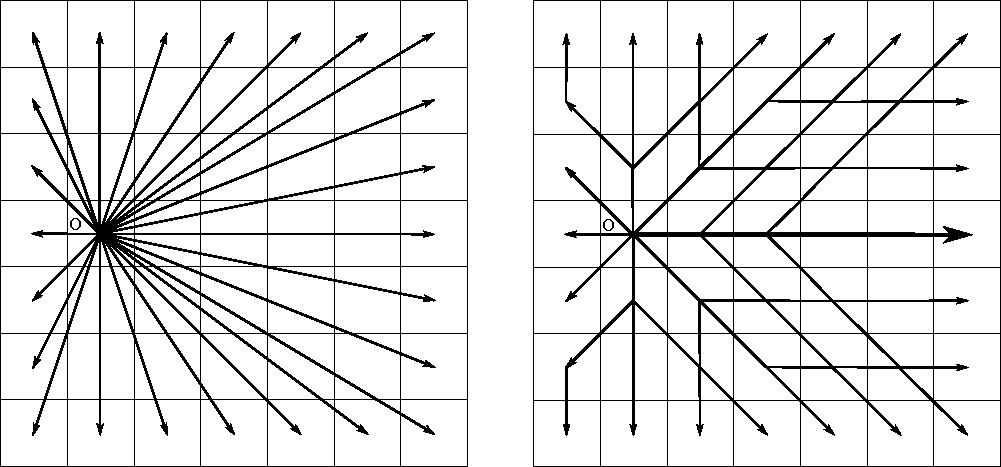
\includegraphics[scale=0.8]{img/grid.pdf} 
	\caption{Rayons lancés sur une image de 7x7 pixels à partir d'un point d'observation situé en (4,2). A gauche, le tracé théorique des rayons, à droite le parcours réel des rayons sur les pixels de l'image.}
	\label{grid}
\end{figure}

Pour chaque rayon, les pixels sont parcourus du plus proche du point O aux plus éloignés. A chaque pixel, l'angle de visé vertical entre le point O et le centre du pixel est calculé. Si l'angle est supérieur aux précédents, le pixel est visible, sinon il ne l'est pas. 

La hauteur des pixels correspond à la somme de l'altitude du MNT et de la hauteur du MNE s'il est présent. La hauteur du point d'observation O correspond à la somme de l'altitude du MNT et du paramètre h1 (Hauteur de l'oeil de l'observateur). La hauteur du MNE n'est jamais prise en compte pour la hauteur de l'observateur (l'observateur ne grimpe pas aux arbres).

La figure \ref{ray_side} représente le calcul d'un rayon sur 5 pixels. Le pixel situé sur le point de l'observateur (pixel 0) est toujours visible. Le pixel suivant (1) est aussi visible, par contre le pixel 2 ne l'est pas car l'angle de visé est plus faible que pour le pixel 1, et ainsi de suite.

\begin{figure}[H]
	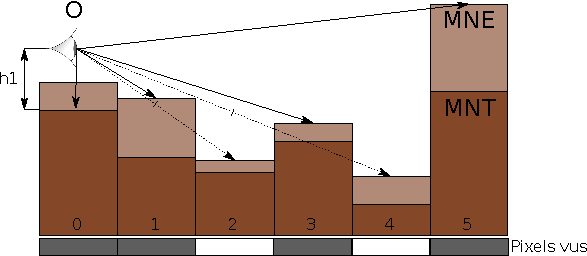
\includegraphics{img/ray_side-fr.pdf} 
	\caption{Vue de profil du lancer d'un rayon.}
	\label{ray_side}
\end{figure}

Le résultat du calcul du rayon de la figure \ref{ray_side} est montré sur la figure suivante (\ref{grid_result}). Il correspond aux pixels de l'image qui sont traversés par le rayon et qui sont visibles depuis le point d'observation.

\begin{figure}[H]
	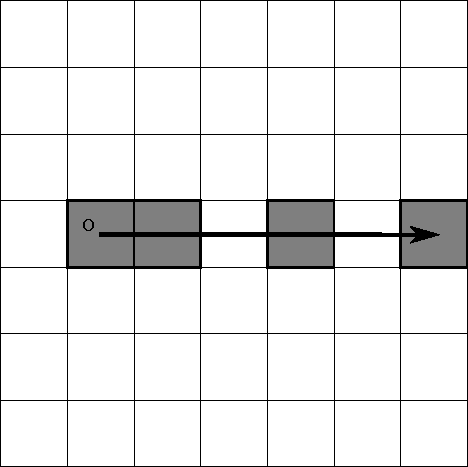
\includegraphics[scale=0.8]{img/grid_result.pdf} 
	\caption{Résultat en vue planimétrique du rayon calculé sur la figure \ref{ray_side}. Les pixels en gris sont les pixels visibles pour ce rayon.}
	\label{grid_result}
\end{figure}

Le résultat complet correspond à la combinaison des résultats pour chaque rayon.
Comme les pixels de l'image peuvent être traversés par des rayons différents, un pixel est marqué visible à partir du moment où il est visible par au moins un des rayons le traversant.

\subsection{Vue planimétrique inverse}

Le mode inverse permet d'inverser l'observateur et l'observé. Le bassin de visibilité n'est plus l'espace visible depuis le point O mais l'espace qui voit le point O. Le point O devient le point observé et l'observateur est positionné sur l'ensemble des points de l'image. La figure \ref{ray_side_inverse} montre le processus pour un rayon donné. 

\begin{figure}[H]
	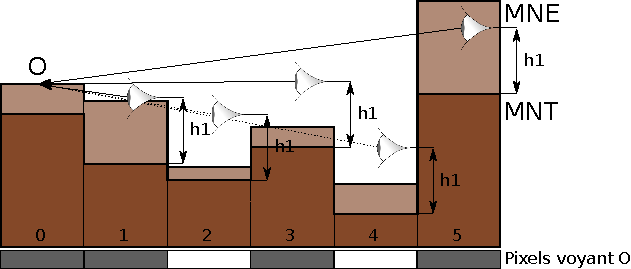
\includegraphics{img/ray_side_inverse-fr.pdf} 
	\caption{Vue de profil du lancer d'un rayon en mode inversé.}
	\label{ray_side_inverse}
\end{figure}

Le résultat est identique ans cet exemple, mais selon la configuration, il peut être différent en vue inverse.

\section{Vue tangentielle}
\label{principles_tan}
Pour la vue tangentielle, le principe de calcul est proche mais comporte quelques différences. Premièrement, le parcours de l'image n'est pas forcément exhaustif. Le nombre de rayons calculés n'est plus dépendant de la taille de l'image mais du paramètre de résolution angulaire $\alpha$. Par défaut, ce paramètre est défini à 0,1°. Le nombre de rayons calculés est de 3600. La figure \ref{grid_tan} montre un exemple avec une précision angulaire de 30°.

\begin{figure}[H]
	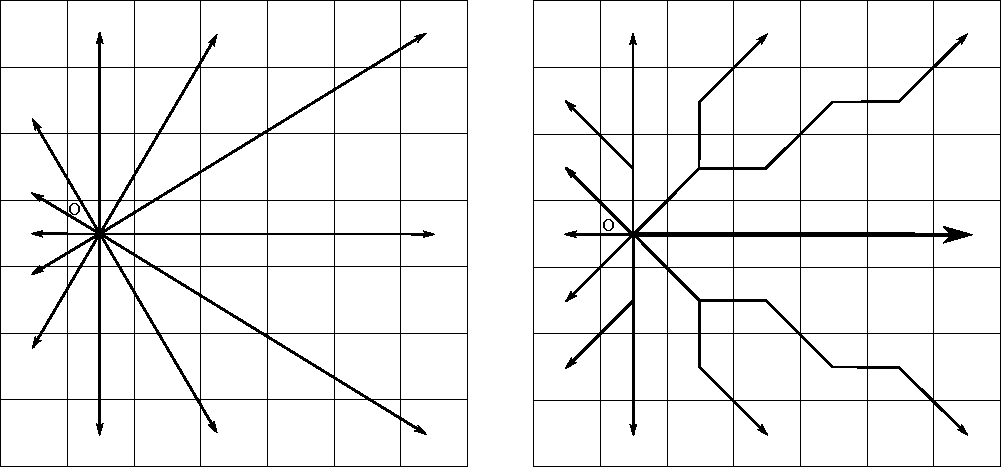
\includegraphics[scale=0.8]{img/grid_tan.pdf} 
	\caption{Rayons lancés sur une image de 7x7 pixels à partir d'un point d'observation situé en (4,2). A gauche, le tracé théorique des rayons, à droite le parcours réel des rayons sur les pixels de l'image. La précision angulaire ($\alpha$) est ici très grossière : 30°.}
	\label{grid_tan}
\end{figure}


Au niveau du calcul de chaque rayon, un traitement supplémentaire doit être réalisé pour déterminer la hauteur d'angle de chaque pixel visible (figure \ref{ray_side_tan}). Le résultat est représenté par la colonne à droite de la figure \ref{ray_side_tan} pour une précision angulaire ($\alpha$) de 10°.

\begin{figure}[H]
	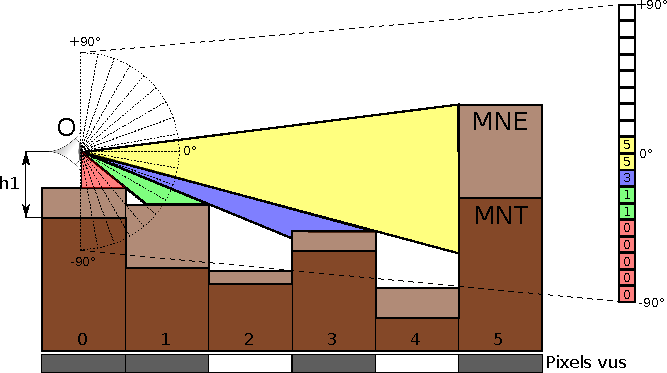
\includegraphics{img/ray_side_tan-fr.pdf} 
	\caption{Vue de profil du lancer d'un rayon. Calcul des hauteurs d'angle des pixels visibles pour la vue tangentielle. La précision angulaire est ici très grossière : 10°.}
	\label{ray_side_tan}
\end{figure}

La juxtaposition des colonnes résultant de chaque rayon forme le résultat de la vue tangentielle. La figure \ref{grid_tan_result} montre le positionnement de chaque rayon calculé dans la vue tangentielle pour une précision angulaire de 30°.

\begin{figure}[H]
	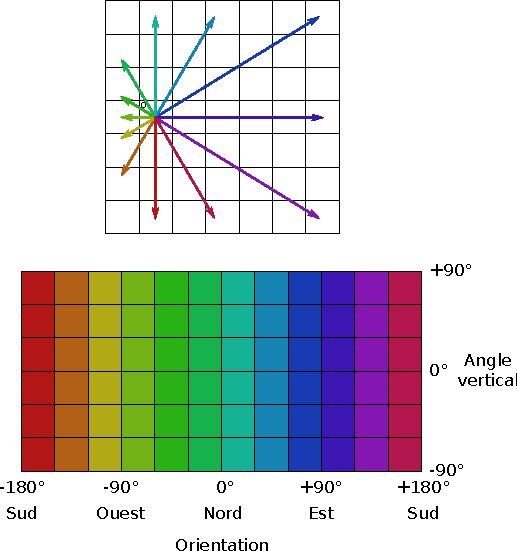
\includegraphics{img/grid_tan_result.pdf} 
	\caption{Position de chaque rayon dans la vue tangentielle résultante. La précision angulaire est ici très grossière : 30°.}
	\label{grid_tan_result}
\end{figure}

\section{Multi-résolution}
\label{multires}
Le calcul en multi-résolution permet d'accélérer fortement les traitements de visibilité. En effet, la complexité algorithmique d'un calcul de visibilité est proportionnel au nombre de pixels de l'image $n$. En multi-résolution, la complexité diminue à $log(n)$ du moment que les résolutions évoluent géométriquement.

\begin{figure}[H]
	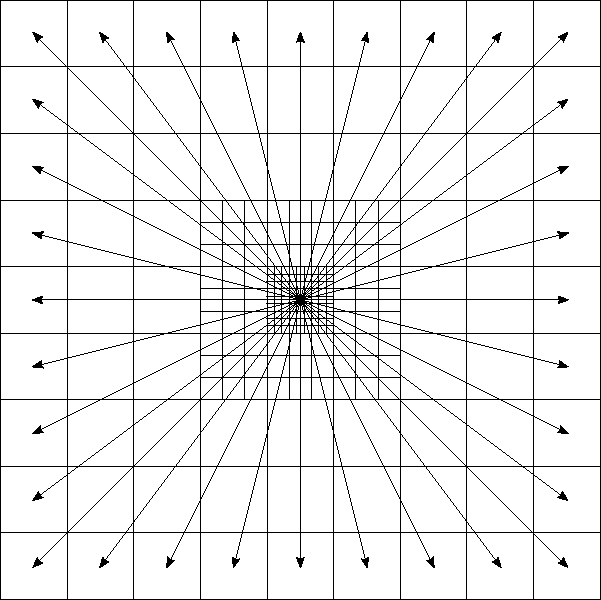
\includegraphics{img/grid_multi.pdf} 
	\caption{Rayons lancés sur une base multi-résolution d'un facteur 3 avec 3 résolutions}
	\label{grid_multi}
\end{figure}

Dans l'exemple de la figure \ref{grid_multi}, le nombre de rayons calculés est de 32 au lieu de 306 et la longueur des rayons en pixel est de 11 au lieu de 41. Le gain en temps de calcul est approximativement de 35 tout en conservant la contrainte de couverture complète de l'espace.


\section{Limitation du champ de vision}
\label{bounds}
Pour tous les calculs de visibilité intégrés dans PixScape, le champ de vision peut être restreint dans les 3 dimensions (figures \ref{bounds_side} et \ref{bounds_2d}) par 6 paramètres : la distance minimale ($d_{min}$) et maximale ($d_{max}$), l'angle vertical minimal ($z_{min}$) et maximal ($z_{max}$) et l'angle horizontal par l'orientation ($orien$) et l'amplitude ($amp$). Les angles sont exprimés en degré dans l'intervalle [0-360] pour les angles horizontaux et [-90;+90] pour les angles verticaux. Les distances sont exprimées en mètre et sont calculées en 2D sur le plan (x,y). 

\begin{figure}[H]
	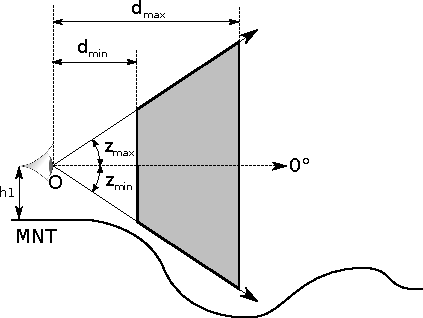
\includegraphics{img/bounds_side.pdf} 
	\caption{Vue de profil des limites du champ de vision}
	\label{bounds_side}
\end{figure}

\begin{figure}[H]
	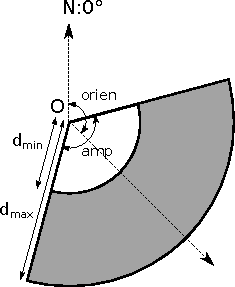
\includegraphics{img/bounds_2d.pdf} 
	\caption{Vue du dessus des limites du champ de vision}
	\label{bounds_2d}
\end{figure}


\chapter{Description des métriques}
\label{metrics}
Dans ce chapitre, l'ensemble des métriques disponibles dans PixScape sont décrites. Le tableau \ref{metrics_tab} liste l'ensemble de ces métriques et ce qu'elles supportent : support des vues planimétrique et/ou tangentielle, support ou non de l'occupation du sol et support des intervalles de distance.

\begin{table}[H]
	\begin{tabular}{|c|c|c|c|c|c|c|}
		\hline
		Métrique & Nom & Planimétrique & Tangentiel & Sans OS & Avec OS & Distance\\
		\hline
		A & Surface & X & X & X & X & X\\
		\hline
		S & Shannon OS & X & X &  & X & X\\
		\hline
		IJI & Interspersion et juxtaposition & X & X &  & X & \\
		\hline
		CONTAG & Contagion & X & X &  & X & \\
		\hline
		DIST & Distribution des distances & X & X & X &  & \\
		\hline
		P & Périmètre & X &  & X &  & \\
		\hline
		C & Compacité & X &  & X &  & \\
		\hline
		FD & Dimension fractale & X &  & X &  & \\
		\hline
		SL & Ligne d'horizon &  & X & X &  & X \\
		\hline
		SD & Shannon distances max. &  & X & X &  & \\
		\hline
		DL & Profondeur de vue &  & X & X &  & \\		
		\hline
	\end{tabular}
	\caption{Liste des métriques et de leur paramétrage}
	\label{metrics_tab}
\end{table}

\section{Métriques communes}

\subsection{Surface : A}
Cette métrique mesure la superficie visible en mètre carré pour la vue planimétrique et en degré carré pour la vue tangentielle. On peut restreindre le calcul à certaines catégories d'occupation du sol et pour différents intervalles de distance.


\subsection{Shannon OS : S}
Cette métrique calcule l'indice de Shannon sur les parts de surface visible de chaque catégorie d'occupation du sol.

$$S = -\frac{1}{\ln n}\sum_{i=1}^{n}\frac{A_i}{A}\ln\left(\frac{A_i}{A}\right)$$

Avec $n$ le nombre de catégories d'occupation du sol, $A_i$ la surface visible de la catégorie $i$ et $A$ la surface totale visible. L'unité des surfaces est en mètre carré pour la vue planimétrique et en degré carré pour la vue tangentielle.

Le projet doit contenir la couche d'occupation du sol pour pouvoir calculer cette métrique.

\subsection{Interspersion et juxtaposition : IJI}
Indice d'interspersion défini dans Fragstat. Dans PixScape, le calcul de cette métrique est appliquée aux surfaces d'occupation du sol visibles.

$$ IJI =  -\frac{100}{\ln 0.5 m(m-1)} \sum_{i=1}^{m} \sum_{k=i+1}^{m}     \dfrac{e_{ik}}{E} \ln \dfrac{e_{ik}}{E}    $$

Le projet doit contenir la couche d'occupation du sol pour pouvoir calculer cette métrique.

\subsection{Contagion : CONTAG}
Indice de contagion défini dans Fragstat. Dans PixScape, le calcul de cette métrique est appliquée aux surfaces d'occupation du sol visibles.

$$ CONTAG = 100 \left[1+\dfrac{1}{2\ln m} \sum _{i=1}^{m}  \sum _{j=1}^{m}  p_i\dfrac{g_{ij}}{\sum _{k=1}^{m}g_{ik} }   \ln \left( p_i\dfrac{g_{ij}}{\sum _{k=1}^{m}g_{ik} }\right)  \right]$$

Le projet doit contenir la couche d'occupation du sol pour pouvoir calculer cette métrique.

\subsection{Distribution des distances : DIST}

La métrique $DIST$ donne un aperçu de la distribution des distances des pixels visibles depuis le point d'observation par quatre opérateurs d'agrégation : la somme, la moyenne, le minimum et le maximum.

Le résultat de la métrique est différent entre la vue tangentielle et planimétrique, les pixels visibles n'étant pas répartis de la même manière entre les deux vues. En effet, en planimétrique, chaque pixel représente une surface au sol en mètre carré, alors qu'en vue tangentielle, chaque pixel représente un cône du champ de vision en degré carré.


\section{Métriques planimétriques}

\subsection{Périmètre : P}

La métrique P correspond au périmètre total du bassin de visibilité, incluant l'ensemble des contours tant extérieur qu'intérieur. L'unité est en mètre.


\subsection{Compacité : C}
Cette métrique reprend l'indice de compacité appliqué au bassin de visibilité complet tel que :

$$C=\frac{P}{2\sqrt{\pi A}}$$

Si $C=1$ le bassin de visibilité est compact \textit{ie.} représente un disque plein. Plus $C$ augmente, moins le bassin de visibilité est compact.


\subsection{Dimension fractale : FD}
Cette métrique calcule la dimension fractale du bassin de visibilité. La méthode utilisée est le box counting.

Le résultat est compris entre 0 et 2. Quand $FD$ tend vers 0 le bassin se réduit à un point, quand $FD$ tend vers 2 le bassin couvre l'espace de façon homogène.

\section{Métriques tangentielles}

\subsection{Ligne d'horizon : SL}

La métrique $SL$ mesure l'aspect plus ou moins accidenté de la ligne d'horizon. Elle est calculée comme le rapport entre la longueur de la ligne d'horizon ($l_h$) et une ligne d'horizon plate ($L=360\deg$). Les longueurs sont exprimées en degré. 

$$SL=\frac{l_h}{L}$$

Quand $SL=1$ l'horizon est plat, plus $SL$ augmente plus la ligne d'horizon est accidentée.

\subsection{Shannon distances max. : SD}
La métrique $SD$ correspond à l’indice de Shannon standardisé appliqué à la distribution des longueurs de vue maximales regroupées en $m$ classes. Les classes de distance sont définies par une suite géométrique : inférieur à 10m, de 10 à 100m, de 100m à 1km, de 1km à 10km, et plus de 10km.

$$SD = -\frac{1}{\ln m}\sum_{i=1}^{m}\frac{nd_i}{n}\ln\left(\frac{nd_i}{n}\right)$$

avec $nd_i$ le nombre de longueurs maximales dans la classe de distance $i$ et $n$ le nombre total de rayons calculés dans la vue tangentielle.

Cette métrique vaut 0 quand toutes les longueurs sont dans la même classe et donc la profondeur de vue est homogène. A l’inverse, elle vaut 1 quand les longueurs de vue sont uniformément réparties dans toutes les classes, ce qui représente une grande variété de profondeurs de vue.

\subsection{Profondeur de vue : DL}
Cette métrique nécessite la construction d’un polygone sur le plan (x,y) regroupant les points visibles les plus éloignés du point d’observation pour chaque rayon lancé. La métrique $DL$ est définie comme l’indice de compacité de ce polygone : 

$$DL=\frac{p}{2\sqrt{\pi a}}$$

où $p$ et $a$ représentent respectivement le périmètre et l’aire du polygone. 

Cette métrique donne une valeur minimale de 1 dans le cas d’un bassin de visibilité de forme circulaire, et des valeurs élevées (non bornées) dans le cas de variations fortes des profondeurs de vue.


\chapter{Performances}
\label{perf}

\section{Parallélisation}
\label{parallelism}
Pour diminuer les temps d'exécution de calcul de visibilité, PixScape implémente 3 méthodes de parallélisation : par thread pour un ordinateur seul, par CUDA pour utiliser l'accélération GPU (Graphics Processor Unit) et par MPI pour les clusters d'ordinateurs.

Le tableau \ref{perf_table} montre les temps d'exécution pour calculer 10000 vues selon le type de vue (planimétrique ou tangentiel), la taille du MNT en million de pixels et la parallélisation : 1 coeur (sans parallélisation), 4 coeurs, 16 coeurs et GPU (carte graphique NVidia Tesla K40).

\begin{table}[htbp]
	
	\begin{tabular}{|l|r|r|r|r|r|}
		\hline
		Type & \multicolumn{1}{l|}{Taille} & \multicolumn{1}{l|}{1 coeur} & \multicolumn{1}{l|}{4 coeurs} & \multicolumn{1}{l|}{16 coeurs} & \multicolumn{1}{l|}{GPU} \\ \hline
		\multicolumn{ 1}{|c|}{Planimétrique} & 1 M & 9,8 & 2,5 & 0,7 & 0,6 \\ \cline{ 2- 6}
		\multicolumn{ 1}{|l|}{} & 9 M & 103,0 & 26,0 & 6,7 & 1,8 \\ \cline{ 2- 6}
		\multicolumn{ 1}{|l|}{} & 100 M & 1168,0 & 376,0 & 83,0 & 13,2 \\ \hline
		\multicolumn{ 1}{|c|}{Tangentiel} & 1 M & 36,0 & 9,8 & 2,7 & 0,8 \\ \cline{ 2- 6}
		\multicolumn{ 1}{|l|}{} & 9 M & 113,0 & 28,8 & 8,0 & 2,2 \\ \cline{ 2- 6}
		\multicolumn{ 1}{|l|}{} & 100 M & 357,0 & 91,0 & 24,7 & 6,3 \\ \hline
	\end{tabular}
	\caption{Temps moyen en minute pour calculer 10000 vues.}
	\label{perf_table}
\end{table}



\subsection{Un ordinateur : threads}
\label{thread}
La parallélisation par thread accélère le calcul sur une seule machine contenant plusieurs cœurs ou processeurs.
Si votre ordinateur a plus qu'un coeur (la plupart), vous pouvez tirer partie de la parallélisation par thread pour accélérer vos calculs avec PixScape. Le temps d'exécution est approximativement inversement proportionnel au nombre de coeurs utilisés. Ce mode de parallélisation est utilisable en interface graphique et en ligne de commande.

\subsubsection{Interface graphique}
La fenêtre "Préferences" accessible par le menu Fichier permet de régler le nombre de coeurs utilisés par PixScape. Il est défini par défaut au nombre coeurs de la machine moins 1. Après avoir modifié le nombre de coeurs utilisé par PixScape, il vaut mieux relancer PixScape pour être sûr que le changement soit bien pris en compte.

\subsubsection{Ligne de commande}
En ligne de commande, il faut définir le nombre de coeurs (ou processeurs) que PixScape peut utiliser avec l'option \verb|-proc| :
\begin{Verbatim}
java -jar pixscape-1.0.jar -proc 8 --project path2myproject/myproject.xml ...
\end{Verbatim}
Par défaut, en ligne de commande, le nombre de coeurs utilisés correspond au nombre défini dans la fenêtre Préférences de l'interface graphique.

En augmentant le nombre de coeurs utilisés par PixScape, vous augmentez, par la même occasion, la taille de la mémoire utilisée par PixScape.

\subsection{Carte graphique : CUDA}
\label{cuda}
Ce mode de parallélisation permet de réaliser les calculs de visibilité sur la carte graphique au lieu du processeur. Les gains en temps d'exécution peuvent être important pour des cartes graphiques Nvidia de la gamme Tesla, conçues pour le calcul haute performance (voir \nameref{perf}). Par contre toutes les métriques ne sont pas optimisées pour le GPU. Les métriques A et S sont les seules à être optimisées. Si vous utilisez d'autres métriques, les gains de temps seront minimes voire inexistant.

Pour pouvoir utiliser l'accélération GPU il faut une carte graphique Nvidia supportant CUDA et que la version 6.5 de CUDA soit installée. 

Si PixScape n'arrive pas à utiliser le GPU, les calculs seront basculés automatiquement sur le processeur.

Ce mode de parallélisation est utilisable en interface graphique et en ligne de commande.

\subsubsection{Interface graphique}

L'activation de l'accélération GPU est accessible à partir de la fenêtre Options (voir \nameref{options}).

En interface graphique, PixScape ne peut utiliser qu'une seule carte graphique, si votre ordinateur contient plusieurs cartes graphiques, PixScape peut les utiliser en parallèle mais uniquement en ligne de commande.

\subsubsection{Ligne de commande}
En ligne de commande, l'option \verb|-cuda| permet d'activer l'utilisation du GPU. Il faut aussi donner le nombre de cartes graphiques à utiliser.

\begin{Verbatim}
java -jar pixscape-1.0.jar -cuda 1 --project path2myproject/myproject.xml ...
\end{Verbatim}
Dans l'exemple ci-dessus, PixScape utilisera une carte graphique pour les calculs de visibilité. Si votre ordinateur contient plusieurs cartes graphiques il est possible d'augmenter le paramètre pour les utiliser en parallèle et diminuer d'autant le temps d'exécution.


\subsection{Cluster : MPI}
PixScape peut aussi être utilisé sur des clusters de calcul supportant Java avec OpenMPI. Ce mode de parallélisation n'est accessible qu'en ligne de commande.

Exemple :
\begin{Verbatim}
mpirun java -jar pixscape-1.0.jar -mpi --project path2myproject/myproject.xml ...
\end{Verbatim}
Seulement certaines commandes peuvent être utilisées dans l'environnement MPI : \verb|--planmetric|, \verb|--tanmetric|, \verb|--landmod|


\section{Gestion mémoire}
\label{memory}
Par défaut, la taille de la mémoire utilisable par PixScape est dépendante du système et peut varier de 128 MB à plusieurs GB.
Si vous avez un gros projets, certaines commandes stopperont le programme à cause d'un manque de mémoire. De plus, si vous utilisez la parallélisation par thread (\nameref{thread}), PixScape aura besoin de plus de mémoire pour chaque coeur utilisé.
Dans tous les cas, si l'exécution se termine par une erreur OutOfMemoryError ou GC overhead, vous devez augmenter la mémoire disponible pour PixScape.

\subsection{Interface graphique}
La mémoire allouée pour PixScape peut être modifiée dans la fenêtre "Préférences" dans le menu Fichier / Préférences. Après avoir changé ce paramètre, PixScape doit être relancé pour qu'il tienne compte de la nouvelle taille mémoire.

En interface graphique, PixScape a besoin de plus de mémoire qu'en ligne de commande du fait de l'affichage des couches. Si vous êtes trop limité en mémoire vive, vous pouvez lancer les calculs en ligne de commande pour diminuer les besoins en mémoire de PixScape (voir \nameref{cli}).

\subsection{Interface en ligne de commande}
Pour définir la mémoire maximale utilisable par PixScape en ligne de commande, il faut utiliser l'option Java \verb|-Xmx| :
\begin{Verbatim}
java -Xmx4g -jar pixscape-1.0.jar ... # 4Gb allocated
java -Xmx1500m -jar pixscape-1.0.jar ... # 1500 Mb -> 1.5Gb allocated
\end{Verbatim}


Si vous ne pouvez pas allouer plus de 1 GB ou 1.5 GB alors que votre ordinateur a plus de mémoire vive, vous utilisez sûrement une version 32-bit de Java qui est limitée à moins de 2 GB.
Pour tester votre version de Java :
\begin{Verbatim}
java -version
\end{Verbatim}
Si vous avez une version 32-bit, installez une version 64-bit de Java pour allouer plus de mémoire à PixScape.


%\section{Multi-résolution}

\end{document}
